\section{Homework Objectives}

The specific objectives of this assignment are as follows \cite{assignment6}:
\begin{itemize}
    \item Get the MNIST and MNIST-C dataset.
    \item Select 3 different types of image corruption (e.g., canny edges) from MNIST-C.
    \item Create mixed datasets for training and test using the original MNIST and corrupted images at a 100/1 ratio for each corruption type.
    \item Create a probability density-based anomaly detector.
    \item Using a range of probability thresholds, create the corresponding ROC and precision-recall curves.
\end{itemize}


\section{Methodology}
\subsection{Data Preparation}
The first step in the assignment was to download the MNIST and MNIST-C datasets. 
We then selected three different types of image corruptions from the MNIST-C dataset.
For each type of corruption, we created a mixed dataset for training and testing. 
This mixed dataset combined the original MNIST images with the corrupted images at a ratio of 100/1. 
This resulted in a dataset that was predominantly composed of normal images, with a small proportion of anomalous (i.e., corrupted) images.\par

Three mixed datasets were created using three seperate selections of corruptions.
The sets of corruptions, chosen randomly, were: "canny, dotted, stripe", "shear, canny, spatter", and "stripe, motion, scale".

\subsection{Visual Review}
We visually reviewed the mixed datasets to ensure that the normal data, fig.~\ref{fig1}, and anomalous images fig(s).~\ref{fig2} through fig(s).~\ref{fig8} were correctly labeled. This step was important to ensure that the anomaly detector was trained on the correct data.\par
\begin{figure}[htbp]
    \centerline{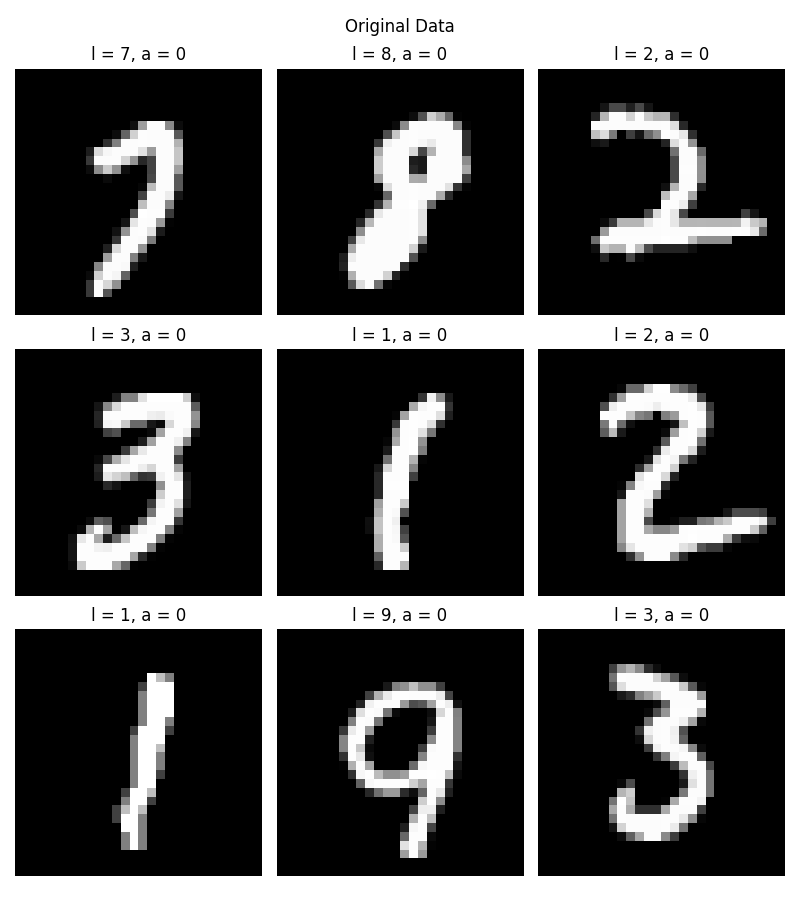
\includegraphics[width=0.5\textwidth]{resources/original_data.png}}
    \caption{Original MNIST data}\label{fig1}
\end{figure}

\begin{figure}[htbp]
    \centerline{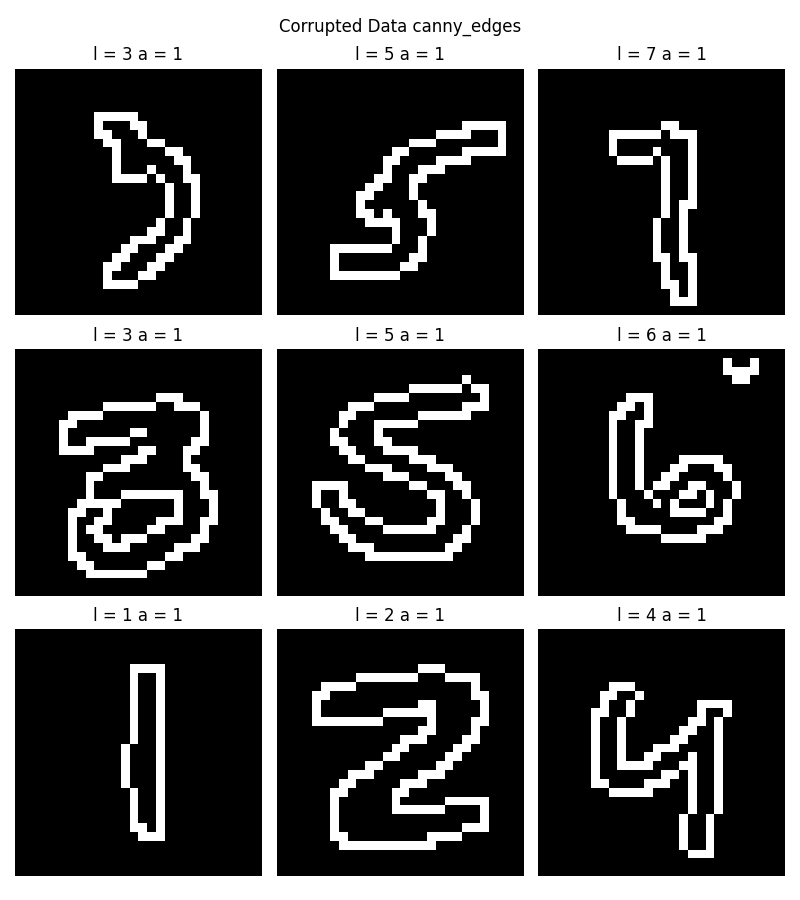
\includegraphics[width=0.5\textwidth]{resources/corrupted_data_canny_edges.png}}
    \caption{MNIST-C, canny edges}\label{fig2}
\end{figure}

\begin{figure}[htbp]
    \centerline{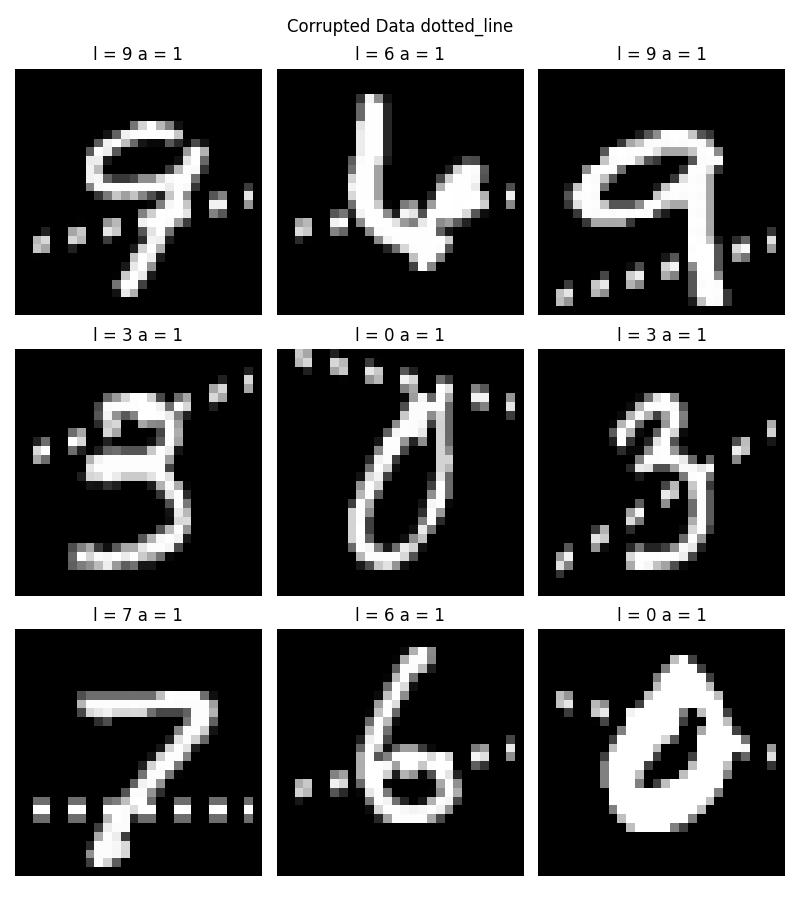
\includegraphics[width=0.5\textwidth]{resources/corrupted_data_dotted_line.png}}
    \caption{MNIST-C, dotted line}\label{fig3}
\end{figure}

\begin{figure}[htbp]
    \centerline{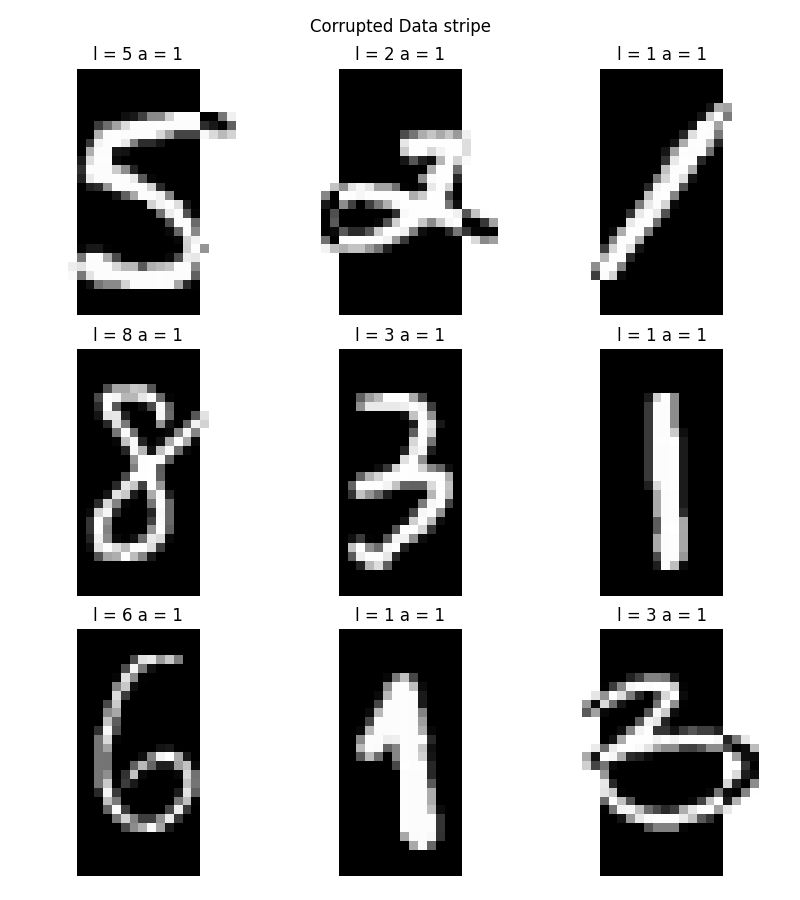
\includegraphics[width=0.5\textwidth]{resources/corrupted_data_stripe.png}}
    \caption{MNIST-C, stripe}\label{fig4}
\end{figure}

\begin{figure}[htbp]
    \centerline{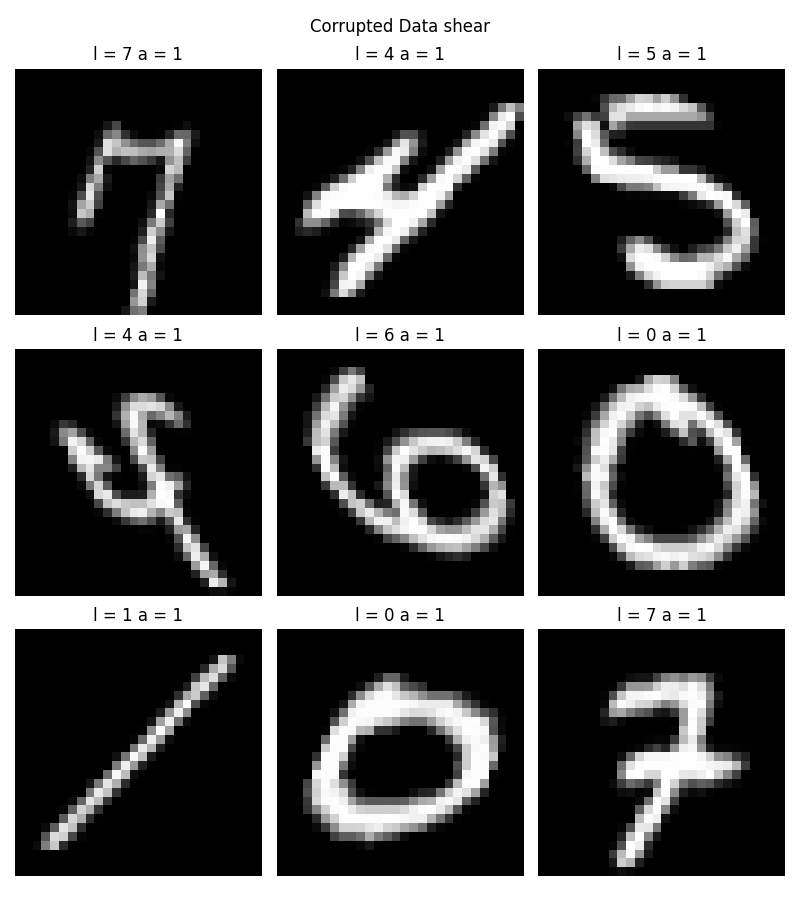
\includegraphics[width=0.5\textwidth]{resources/corrupted_data_shear.png}}
    \caption{MNIST-C, shear}\label{fig5}
\end{figure}

\begin{figure}[htbp]
    \centerline{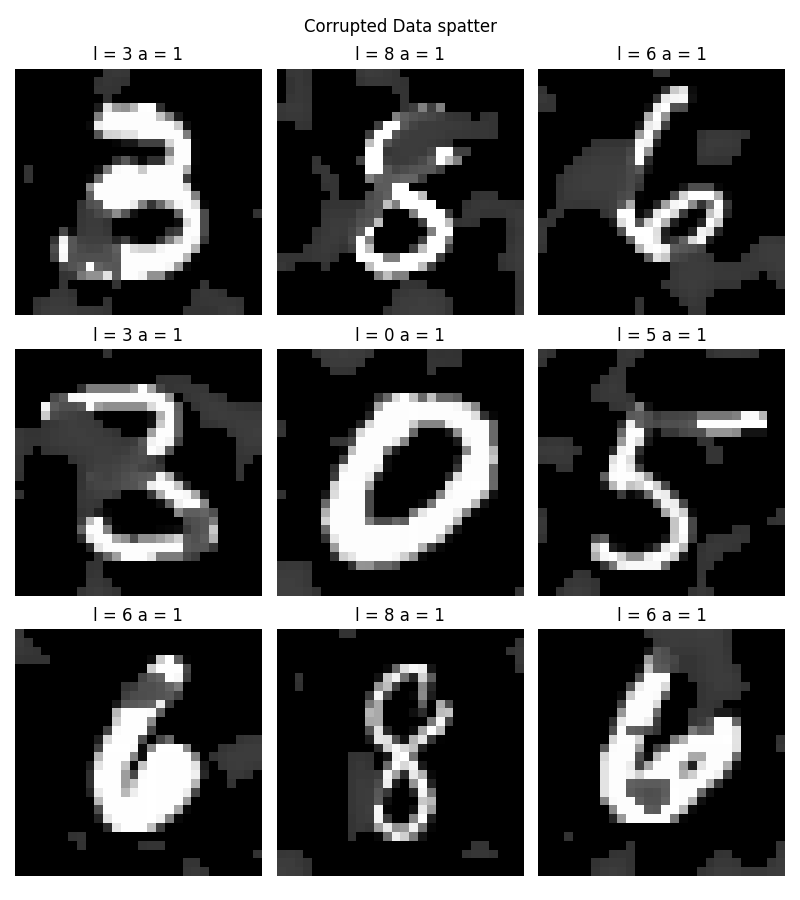
\includegraphics[width=0.5\textwidth]{resources/corrupted_data_spatter.png}}
    \caption{MNIST-C, spatter}\label{fig6}
\end{figure}

\begin{figure}[htbp]
    \centerline{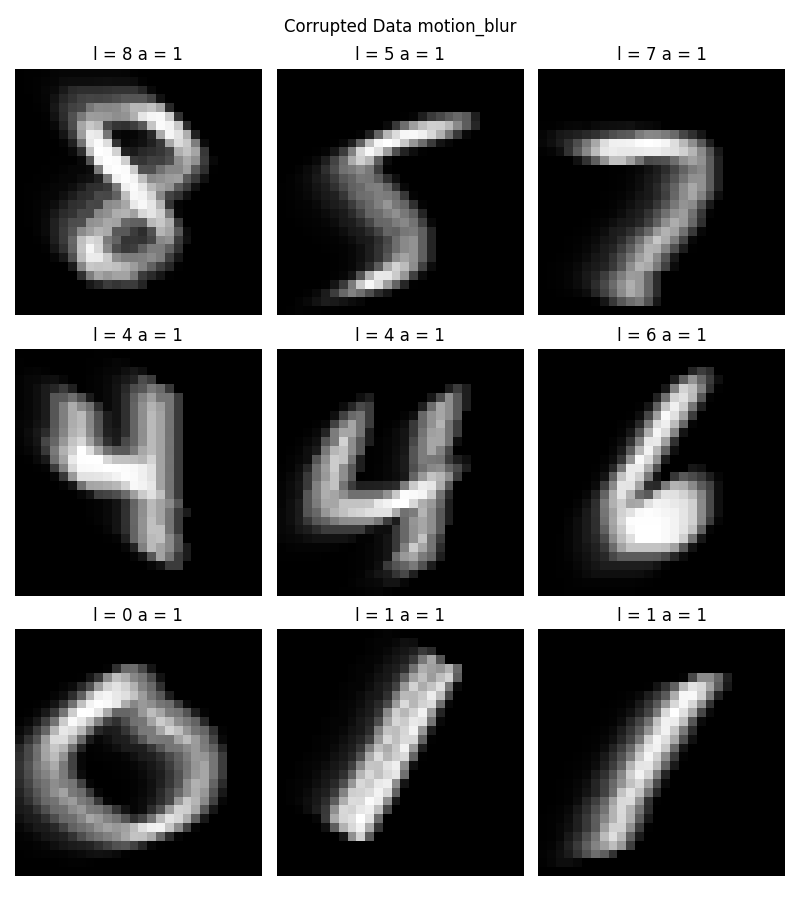
\includegraphics[width=0.5\textwidth]{resources/corrupted_data_motion_blur.png}}
    \caption{MNIST-C, motion blur}\label{fig7}
\end{figure}

\begin{figure}[htbp]
    \centerline{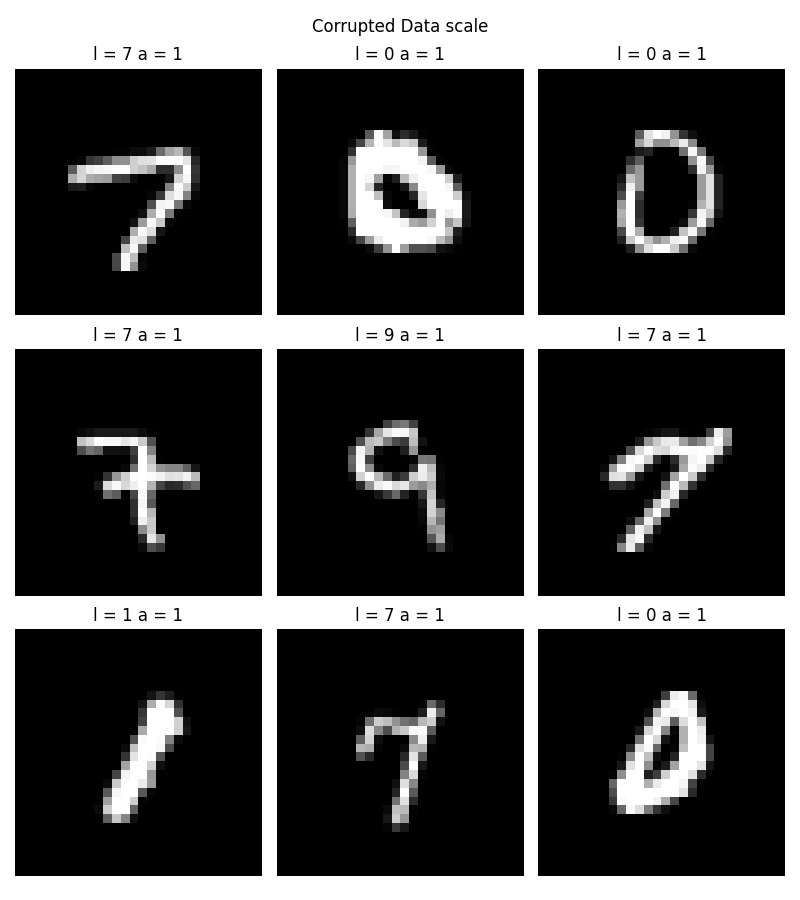
\includegraphics[width=0.5\textwidth]{resources/corrupted_data_scale.png}}
    \caption{MNIST-C, scale}\label{fig8}   
\end{figure}


\subsection{Anomaly Detection}
We implemented a probability density-based anomaly detector using the implementation from scikit-learn of K-Nearest Neighbors (KNN) and Random Forest(RF). 
This is a supervised learning algorithm where labels of anomaly and normal data are used to train the model.
The anomaly label is 1 for anomalous data and 0 for nominal data.\par

\subsection{Performance Evaluation}
We evaluated the performance of the anomaly detector using ROC and PR curves. 
The ROC curve plots the true positive rate against the false positive rate at different probability thresholds.
A true positive is an instance where the model correctly predicts the positive class, while a false positive is an instance where the model incorrectly predicts the positive class.\par
The PR curve plots the precision against the recall at different probability thresholds. 
Precision is the ratio of true positives to the sum of true positives and false positives, while recall is the ratio of true positives to the sum of true positives and false negatives.\cite{precision_recall_wiki}\par
These curves provide a visual representation of the trade-off between true positives and false positives, and between precision and recall, respectively.\par








